При разработке микро-сервиса рекомендательной системы была разработана следующая
архитектура:
\begin{figure}[H]
    \centering
    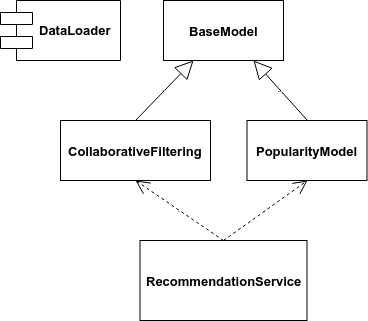
\includegraphics[scale=0.8]{images/classes.png}
    \caption{Структура классов рекомендательной системы}
\end{figure}

\textbf{DataLoader}

Данный модуль отвечает за выгрузку истории заказов из базы данных, а также за
их обработку.

\textbf{BaseModel}

Базовый класс, описывающий модель рекомендательной системы. В нем реализованы общие
функции для всех моделей.

\textbf{CollaborativeFiltering}

Класс, отвечающий за модель коллаборативной фильтрации. Является базовым
для \textit{ItemCollaborativeFiltering} и \textit{CompanyCollaborativeFiltering},
классы коллаборативной фильтрации для блюд и компаний соответственно.

\textbf{PopularityModel}

Класс, отвечающий за модель "Популярное". Является базовым
для \textit{ItemPopularityModel} и \textit{CompanyPopularityModel},
классы моделей для блюд и компаний соответственно.

Описание всех алгоритмов приводится в книге Recommender Systems
Handbook \cite{RSHandbook}.
